\documentclass[12pt,a4paper,twocolumn]{article}
% The following LaTeX packages must be installed on your machine: amsmath, authblk, bm, booktabs, caption, dcolumn, fancyhdr, geometry, graphicx, hyperref, latexsym, natbib
\input{151.dat}
\usepackage{gensymb}
\usepackage{float}
\usepackage{siunitx}
\usepackage{amssymb}
\usepackage{float}
\usepackage{listings}
\PassOptionsToPackage{hyphens}{url}\usepackage{hyperref}
\usepackage[none]{hyphenat}
%\renewcommand{\familydefault}{\sfdefault}


\begin{document}

\setcounter{page}{1}

\section*{Problem 1.2}

\paragraph{(a)}
Based on the situations presented in Problem 1.1, we expect that the number of particles $n(t)$ in the left side of the box will decrease within a transient time period as they distribute themselves equally within the box, and oscillate around some value when it reaches steady state.

\paragraph{(b)}
In agreement with (a), $n(t)$ does indeed approach equilibrium in the form of oscillation about some value. This value turns out to be the mean value of the number of particles in a partition over time. As the number of particles $N$ is increased, the oscillations about the mean become smaller and equilibrium is better defined. This definition of equilibrium is independent of the initial distribution of the particles in the box.

\paragraph{(c)}
As stated in (b), the number of particles in a partition is not constant, but rather oscillates around the mean number of particles in that partition over time.

\paragraph{(d)}
For $N \geq 32$, the system does not return to its initial state, since we have set the initial state to be all the particles confined in one partition, which is certainly not an equilibrium state.

\paragraph{(e)}
The mean number $\bar{n}$ of particles on the left partition in the equilibrium state is roughly $N/2$. Since the program calculates this value starting at $t = 0$, the exact value will not be correct since the mean value during the transient period will bias the average towards a value higher than $N/2$. Zeroing the averages after the system reaches steady state shows the correct value, very close to $N/2$.

\paragraph{(f)}
$\sigma$ is known as the standard deviation, and is a measure of the displacement of each state from the mean value. If $n$ were constant, $\sigma$ would be zero. The ratio $\sigma/\bar{n}$ is known as the standard deviation of the mean, and is a measure of the relative fluctuations of $n$. The greater $N$ is, the smaller $\sigma/\bar{n}$ becomes.

\begin{figure}[htb]
	\centering
	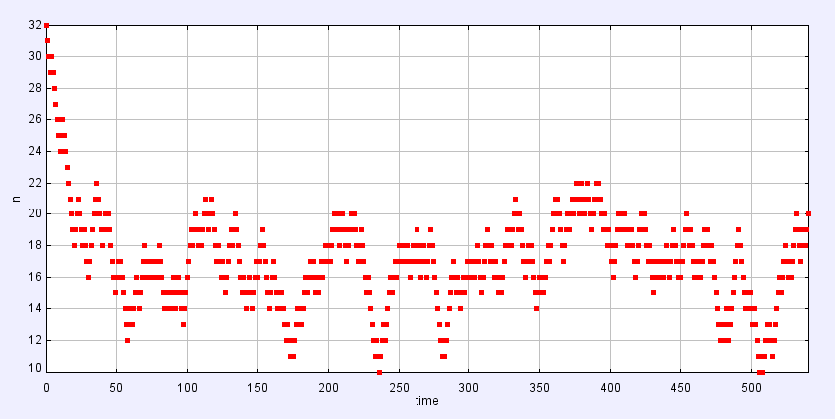
\includegraphics[width=0.45\textwidth]{equi2.png}
	\caption{Approach to equilibrium, $N = 32$. Equilibrium is achieved at around $t = 50$, where $n(t)$ starts to oscillate around the mean value 16.}
	\label{fig:gas}
\end{figure}


\end{document}